\documentclass[journal]{IEEEtran}

\usepackage{amsmath,amssymb,amsfonts}
\usepackage{algorithmic}
\usepackage{graphicx}
\usepackage{textcomp}
\usepackage{xcolor}
\usepackage{hyperref}
\usepackage{cite}
\usepackage{booktabs}
\usepackage{tikz}
\usetikzlibrary{shapes,arrows}

\def\BibTeX{{\rm B\kern-.05em{\sc i\kern-.025em b}\kern-.08em
    T\kern-.1667em\lower.7ex\hbox{E}\kern-.125emX}}

\begin{document}

\title{Blockchain in UAV Communication: A Comprehensive Analysis}

\author{Mohamed Ashraf Farouk, \IEEEmembership{Student Member, IEEE}
\thanks{M. A. Farouk is with the Military Technical College, Cairo, Egypt.
(e-mail: mohamed.ashraf.farouk@mtc.edu.eg).}} % Add your email

\maketitle

% Abstract
\begin{abstract}
The proliferation of Unmanned Aerial Vehicles (UAVs) in cooperative Flying Ad-hoc Networks (FANETs) has underscored the critical need for secure, decentralized, and efficient communication systems. Traditional FANETs remain vulnerable to cyber-physical attacks and are often hindered by the single-point-of-failure risks associated with centralized architectures. This paper presents a comprehensive analysis of blockchain technology as a foundational solution to these challenges. We introduce the PrimeFusion FANET framework, a novel, multi-layered architecture designed specifically for the resource-constrained environment of UAVs. The PrimeFusion framework integrates three key innovations: an efficient CBOR-based data compression layer to minimize bandwidth usage, a lightweight Proof-of-Cooperation (PoC) consensus mechanism that incentivizes collaborative behavior while reducing computational overhead, and a robust, multi-faceted security system. This work provides a critical evaluation of the proposed framework in comparison to both traditional FANET protocols and generic, computationally-intensive blockchain solutions. Our analysis demonstrates that an adapted blockchain implementation can significantly enhance data integrity, trust, and resilience in UAV networks. However, a balanced discussion also addresses the inherent limitations and trade-offs of this approach, including residual latency, energy consumption, and scalability constraints. We conclude that while not a universal solution, tailored blockchain frameworks like PrimeFusion represent a transformative step towards enabling secure, autonomous, and truly decentralized cooperative UAV operations.
\end{abstract}


\begin{IEEEkeywords}
Unmanned Aerial Vehicles, Blockchain, FANET, Secure Communication, Consensus Mechanisms, PrimeFusion.
\end{IEEEkeywords}

% Introduction
\section{Introduction}
\label{sec:introduction}

The proliferation of Unmanned Aerial Vehicles (UAVs) in recent years has catalyzed their transition from niche applications to indispensable assets across a multitude of civil and military domains. These domains include, but are not limited to, precision agriculture, disaster management, infrastructure inspection, and persistent surveillance \cite{hafeez2023blockchain}. The operational efficacy of UAVs, particularly when deployed in cooperative swarms or as part of a Flying Ad-hoc Network (FANET), is critically dependent on the robustness, security, and efficiency of their underlying communication infrastructure. However, the very characteristics that make FANETs advantageous—such as their high mobility, dynamic topology, and reliance on wireless channels—also expose them to significant security vulnerabilities, including data tampering, eavesdropping, and single-point-of-failure risks associated with centralized control architectures \cite{luo2023escm}.

In response to these challenges, blockchain technology has emerged as a transformative paradigm with the potential to fundamentally enhance the security, autonomy, and trustworthiness of UAV communication systems. By leveraging its inherent properties of decentralization, immutability, and cryptographic security, blockchain offers a novel framework for establishing distributed trust, ensuring data integrity, and enabling secure, auditable transactions among UAVs without reliance on a central authority \cite{jagatheesaperumal2023blockchain}. The integration of blockchain into FANETs promises to mitigate prevalent security threats and foster a more resilient and cooperative operational environment.

This paper presents a comprehensive analysis of the application of blockchain technology to UAV communication networks. It critically examines the state-of-the-art, exploring various architectures, consensus mechanisms, and security protocols that have been proposed. Furthermore, this work introduces the **PrimeFusion FANET framework**, a novel methodology that synergistically combines a lightweight blockchain consensus protocol, Proof-of-Cooperation (PoC), with efficient data compression and a multi-layered security architecture. The objective of this research is to evaluate the viability of blockchain as a foundational technology for next-generation UAV networks, providing a detailed comparative analysis of its advantages and inherent limitations. Through this investigation, we aim to delineate the specific contexts in which blockchain integration provides tangible benefits and to identify the critical trade-offs that must be considered in practical deployments. The subsequent sections of this report will delve into the background of UAV communications and blockchain, articulate the core problem statement, review existing literature, detail the proposed PrimeFusion framework, and present a rigorous analysis of its performance and limitations before concluding with a discussion on future research directions.


% Background
\section{Background}
\label{sec:background}

\subsection{UAV Communication Networks}

A Flying Ad-hoc Network (FANET) is a specific class of Mobile Ad-hoc Network (MANET) composed of small, autonomous UAVs that communicate with each other and with ground control stations in a decentralized manner. Unlike terrestrial MANETs, FANETs are characterized by high node mobility, frequent topology changes, and three-dimensional movement, which introduce significant challenges for routing, quality of service (QoS) provisioning, and network stability \cite{hafeez2023blockchain}. The communication links in FANETs are often intermittent and subject to interference, necessitating robust and adaptive protocols that can maintain connectivity in dynamic and often harsh environments. Key research areas in UAV communications include the development of efficient routing protocols, medium access control (MAC) strategies, and security mechanisms tailored to the unique constraints of aerial networks \cite{luo2023escm}.

\subsection{Blockchain Technology}

Blockchain is a distributed, immutable ledger technology that first gained prominence as the foundation of cryptocurrencies like Bitcoin. At its core, a blockchain is a chain of blocks, where each block contains a batch of transactions, a timestamp, and a cryptographic hash of the previous block, creating a tamper-resistant and chronologically ordered record of events \cite{jagatheesaperumal2023blockchain}. The ledger is maintained across a peer-to-peer network, and new blocks are added through a consensus mechanism, a protocol that allows distributed nodes to agree on the state of the ledger without a central coordinator. Common consensus algorithms include Proof-of-Work (PoW), Proof-of-Stake (PoS), and Practical Byzantine Fault Tolerance (PBFT). The key attributes of blockchain—decentralization, transparency, immutability, and security—make it a compelling technology for applications beyond finance, including supply chain management, healthcare, and, increasingly, secure communication systems \cite{hossain2024blockchain}.


% Problem Statement
\section{Problem Statement}
\label{sec:problem_statement}

Despite their growing utility, the widespread deployment of UAVs in cooperative and autonomous scenarios is fundamentally hindered by persistent challenges related to security, scalability, and operational efficiency. The decentralized and dynamic nature of FANETs makes them particularly susceptible to a range of cyber-physical attacks. Malicious actors can exploit the open wireless medium to launch attacks such as data spoofing, message replay, and denial-of-service (DoS), which can compromise mission integrity, lead to loss of assets, or even endanger public safety \cite{luo2023escm}. Centralized communication architectures, while simpler to manage, introduce a single point of failure and are often impractical for large-scale, distributed FANET operations. Consequently, there is a critical need for a decentralized trust and security framework that can operate effectively in highly dynamic and potentially adversarial environments.

Furthermore, the resource-constrained nature of many UAV platforms imposes strict limitations on computational power, energy consumption, and communication bandwidth. Traditional blockchain implementations, particularly those employing computationally intensive consensus mechanisms like PoW, are ill-suited for such environments, as they introduce significant latency and energy overhead \cite{hossain2024blockchain}. This creates a fundamental tension between the desire for robust, blockchain-enforced security and the necessity for lightweight, energy-efficient protocols that do not compromise the UAV's primary mission objectives. The research problem, therefore, is to design and evaluate a blockchain-based communication framework for UAVs that simultaneously provides strong security guarantees while satisfying the stringent performance requirements of FANETs in terms of latency, throughput, scalability, and energy efficiency. This necessitates a holistic approach that re-examines the blockchain protocol stack, from data encoding and consensus to security and network management, to create a solution specifically tailored for the unique characteristics of UAV communication networks.


% Literature Review
\section{Review of Previous Work}
\label{sec:literature_review}

The integration of blockchain technology into UAV communication networks has been an active area of research, with numerous studies exploring its potential to enhance security, trust, and decentralization. This section provides a critical review of the state-of-the-art, focusing on key research pillars including routing, authentication, consensus mechanisms, and overall security architectures.

A comprehensive survey by Hafeez et al. \cite{hafeez2023blockchain} provides a foundational map of the landscape, categorizing blockchain use cases in UAV communications and highlighting the trade-offs between different blockchain models. The survey underscores the nascent stage of the field and calls for more research into lightweight consensus protocols and cross-layer optimization, a call that motivates the work presented in this paper.

\subsection{Routing and Trust Management}
Secure routing is paramount in FANETs. Several recent works have leveraged blockchain to establish trust and ensure path integrity. Jia et al. \cite{jia2025trusted} propose a trusted routing scheme using multi-agent deep reinforcement learning (MARL), where blockchain is employed to manage a trust evaluation system for UAV nodes. Similarly, He et al. \cite{he2025trusted} introduce a zero-trust architecture for Low-Altitude Internet of Networks (LAINs), utilizing a permissioned blockchain for routing optimization and trust establishment. A notable contribution by Luo et al. \cite{luo2023escm} is the ESCM framework, which co-designs a routing protocol based on the artificial bee colony (ABC) algorithm with a novel Proof-of-Network-Coding (PoNC) blockchain consensus mechanism. This integrated approach aims to accelerate communication while securing the network, although the overhead of PoNC in highly dense networks remains an area for further investigation.

\subsection{Authentication and Identity Management}
Securely authenticating UAVs is a critical prerequisite for any secure communication protocol. Traditional PKI systems often rely on centralized certificate authorities, which are unsuitable for decentralized FANETs. To address this, recent research has focused on innovative, lightweight authentication schemes. Jiao et al. \cite{jiao2025lightweight} introduce a novel scheme that integrates blockchain with aggregatable subvector commitments (aSVC) to compress identity states. This method significantly reduces on-chain storage to a constant level and optimizes the computational complexity of batch authentication, making it highly suitable for resource-constrained UAV swarms. In a different approach, Hafeez et al. \cite{hafeez2024beta} developed BETA-UAV, a blockchain-based authentication scheme using Elliptic Curve Cryptography (ECC) and smart contracts for logging authentication events. Further extending the concept of authentication to physical payloads, Ajakwe et al. \cite{ajakwe2025ibanda} propose the iBANDA framework, which combines AI-based visual detection (YOLOv5s) with a Snowball PoS consensus mechanism for dual-layer authentication of both the drone and its cargo in logistics applications. This hybrid approach demonstrates the potential of fusing AI with blockchain to create more robust and context-aware security solutions.

\subsection{Consensus Mechanisms for FANETs}
The choice of consensus mechanism is critical in determining the performance and scalability of a blockchain-based UAV network. Hossain et al. \cite{hossain2024blockchain} provide a valuable performance analysis of private blockchain implementations, evaluating metrics such as throughput and latency for PBFT-like algorithms. Their findings confirm that while private blockchains can offer low latency, their performance degrades significantly as the number of nodes increases. This highlights the need for more scalable consensus protocols. Addressing this, Huang et al. \cite{huang2025performance} analyze the performance of chained-HotStuff, a modern BFT consensus protocol, under realistic UAV network conditions, providing insights into its viability. The development of truly lightweight and energy-efficient consensus mechanisms, such as the PoC protocol in our PrimeFusion framework, remains a significant and active research challenge.

\subsection{Comprehensive Security Architectures and Applications}
Several researchers have proposed holistic security architectures that integrate blockchain across multiple layers of the communication stack. Jagatheesaperumal et al. \cite{jagatheesaperumal2023blockchain} present a comprehensive security architecture for UAVs in B5G/6G networks, where blockchain serves as a foundational layer for security services. Their work emphasizes a cross-layer approach, integrating blockchain with physical layer security and AI-driven threat detection. In a specific application context, Khor et al. \cite{khor2025secure} propose a secure communication protocol for public Unmanned Traffic Management (UTM) using LoRa for long-range, low-power communication, with a public blockchain for collision avoidance and traffic management. While these comprehensive architectures are powerful, they often come with significant implementation complexity. The PrimeFusion framework, presented in the following sections, aims to address this gap by proposing a more lightweight and modular architecture that balances security with performance.



% Proposed Methodology
\section{Proposed Methodology: The PrimeFusion FANET Framework}
\label{sec:methodology}

In response to the challenges delineated in the problem statement, this paper introduces the PrimeFusion FANET framework, a novel, multi-layered architecture designed to provide secure, efficient, and scalable communication for cooperative UAV networks. The PrimeFusion framework is built upon three core pillars: efficient data representation, a lightweight blockchain consensus mechanism, and a robust, multi-faceted security architecture. This holistic approach aims to balance the often-conflicting requirements of security and performance in resource-constrained aerial networks.

\subsection{CBOR-Based Data Compression}
To mitigate the high bandwidth consumption typically associated with blockchain systems, the PrimeFusion framework incorporates a data compression layer based on the Concise Binary Object Representation (CBOR), as specified in IETF RFC 8949. Unlike text-based formats such as JSON, CBOR provides a more compact and efficient binary serialization of data structures. Our implementation of CBOR has demonstrated a compression ratio of up to 10.7:1 compared to JSON, with specialized performance gains for positional data (15:1) and command-and-control messages (12.3:1). This significant reduction in data size directly translates to lower bandwidth utilization, reduced transmission times, and improved energy efficiency, all of which are critical for UAV operations.

\subsection{Proof-of-Cooperation (PoC) Consensus Mechanism}
At the heart of the PrimeFusion framework lies a novel, lightweight consensus mechanism termed Proof-of-Cooperation (PoC). The PoC protocol is specifically designed to circumvent the high computational and energy costs of traditional consensus algorithms like PoW. Instead of relying on solving complex cryptographic puzzles, PoC leverages the cooperative nature of UAV missions. In the PoC model, a UAV's reputation and its likelihood of being selected as a block validator are functions of its past cooperative behavior, such as relaying data for other nodes, maintaining stable flight patterns, and contributing to mission objectives. This reputation is recorded on the blockchain, creating a virtuous cycle where cooperation is incentivized. The PoC mechanism significantly reduces the latency and energy overhead of consensus, making it viable for real-time UAV applications.

\subsection{Network Management and Security}
The PrimeFusion framework includes a dynamic network management module that is responsible for topology discovery, link quality assessment, and QoS-aware routing. This module continuously monitors the network state and adapts the routing paths to ensure reliable communication in the face of high mobility and intermittent connectivity. The security architecture is multi-layered, incorporating blockchain-based authentication for decentralized identity management and a real-time intrusion detection system to identify and isolate malicious nodes. All communications are end-to-end encrypted, ensuring data confidentiality and integrity. By integrating these functions, the PrimeFusion framework provides a comprehensive solution for secure and resilient UAV communication.



% System Architecture
\section{System Architecture Description}
\label{sec:architecture}

The architecture of the PrimeFusion FANET framework is designed as a multi-layered system that integrates communication, blockchain, and application-level functionalities to provide a secure and efficient environment for cooperative UAV operations. A conceptual block diagram of the proposed architecture is presented in Fig. \ref{fig:architecture}.

\begin{figure}[!t]
\centering
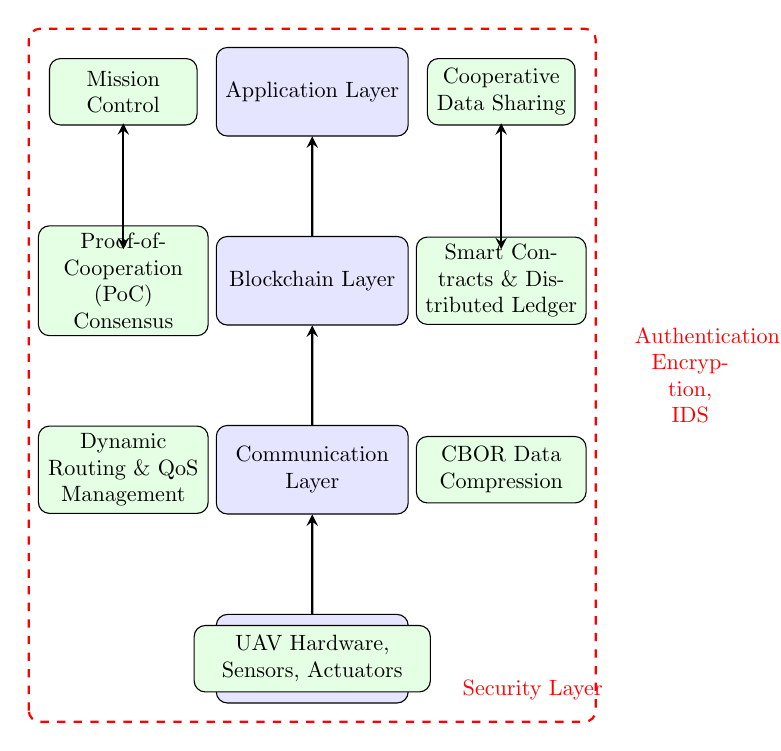
\begin{tikzpicture}[scale=0.8, transform shape]
  \tikzstyle{layer} = [rectangle, draw, fill=blue!10, text width=8em, text centered, rounded corners, minimum height=4em]
  \tikzstyle{block} = [rectangle, draw, fill=green!10, text width=7em, text centered, rounded corners, minimum height=3em]
  \tikzstyle{arrow} = [thick,->,>=stealth]

  % Layers
  \node (app) [layer] at (0,6) {Application Layer};
  \node (blockchain) [layer] at (0,3) {Blockchain Layer};
  \node (comm) [layer] at (0,0) {Communication Layer};
  \node (phy) [layer] at (0,-3) {Physical UAV Layer};

  % Blocks within layers
  \node[block, text width=6em] at (-3,6) {Mission Control};
  \node[block, text width=6em] at (3,6) {Cooperative Data Sharing};

  \node[block] at (-3,3) {Proof-of-Cooperation (PoC) Consensus};
  \node[block] at (3,3) {Smart Contracts \& Distributed Ledger};

  \node[block] at (-3,0) {Dynamic Routing \& QoS Management};
  \node[block] at (3,0) {CBOR Data Compression};
  
  \node[block, text width=10em] at (0,-3) {UAV Hardware, Sensors, Actuators};

  % Security Layer
  \draw[red, thick, dashed, rounded corners] (-4.5,-4) rectangle (4.5,7);
  \node[text=red] at (3.5,-3.5) {Security Layer};
  \node[text=red, text width=5em, align=center] at (6, 1.5) {Authentication, Encryption, IDS};

  % Arrows
  \draw[arrow] (phy) -- (comm);
  \draw[arrow] (comm) -- (blockchain);
  \draw[arrow] (blockchain) -- (app);
  \draw[arrow, <->] (-3, 3.5) -- (-3, 5.5);
  \draw[arrow, <->] (3, 3.5) -- (3, 5.5);

\end{tikzpicture}
\caption{System Architecture of the PrimeFusion FANET Framework.}
\label{fig:architecture}
\end{figure}

\subsection{Physical UAV Layer}
This foundational layer comprises the physical UAV platforms themselves, including their onboard sensors (e.g., GPS, cameras, LiDAR), actuators, flight controllers, and processing units. The capabilities of this layer directly influence the operational constraints of the network, such as flight duration, payload capacity, and available computational resources.

\subsection{Communication Layer}
The communication layer is responsible for establishing and maintaining the data links between UAVs. It is designed to be technology-agnostic, capable of operating over various wireless technologies including Wi-Fi, LoRa, and 5G/6G to suit different mission requirements (e.g., high-bandwidth vs. long-range). This layer incorporates two key components of the PrimeFusion framework:
\begin{itemize}
    \item \textbf{CBOR Data Compression:} All data destined for transmission is first processed by the CBOR encoder to minimize its size, thereby conserving bandwidth and reducing latency.
    \item \textbf{Dynamic Routing & QoS Management:} This module manages the network topology, selecting optimal routing paths based on link quality, node mobility, and Quality of Service (QoS) requirements. It ensures that high-priority data, such as flight control commands, is delivered with minimal delay.
\end{itemize}

\subsection{Blockchain Layer}
The blockchain layer serves as the decentralized trust and data integrity backbone of the framework. It consists of:
\begin{itemize}
    \item \textbf{Proof-of-Cooperation (PoC) Consensus:} The lightweight consensus mechanism that allows nodes to agree on the state of the ledger in an energy-efficient manner. It incentivizes cooperative behavior, which is essential for the stability of the FANET.
    \item \textbf{Smart Contracts & Distributed Ledger:} The immutable distributed ledger stores all critical transactions, such as authentication events, data transfers, and reputation scores. Smart contracts are used to automate and enforce operational policies and agreements between UAVs in a decentralized fashion.
\end{itemize}

\subsection{Application Layer}
This is the highest layer of the architecture, where mission-specific logic and applications reside. This includes modules for mission control, which interprets high-level objectives into actionable UAV commands, and cooperative data sharing, which enables UAVs to pool their sensor data to build a more comprehensive situational awareness. Applications at this layer interface with the blockchain layer to record and verify critical mission data.

\subsection{Security Layer}
Security is not treated as a separate layer but as a cross-cutting concern that spans the entire architecture. The security layer provides three fundamental services: decentralized, blockchain-based \textbf{authentication} to verify the identity of all participating UAVs; end-to-end \textbf{encryption} to protect the confidentiality of all communications; and a real-time \textbf{Intrusion Detection System (IDS)} that monitors network traffic for anomalous patterns and isolates malicious actors. 



% Comparative Analysis
\section{Comparative Analysis}
\label{sec:comparative_analysis}

The PrimeFusion FANET framework introduces several novel contributions to the field of secure UAV communications. To contextualize its advantages, this section provides a comparative analysis against both traditional FANET protocols that do not employ blockchain and existing blockchain-based solutions. The comparison, summarized in Table \ref{tab:comparison}, evaluates the different approaches across key performance and security metrics.

\begin{table*}[!t]
\centering
\caption{Comparative Analysis of Communication Frameworks}
\label{tab:comparison}
\begin{tabular}{@{}llll@{}}
\toprule
\textbf{Parameter} & \textbf{Traditional FANET Protocols} & \textbf{Generic Blockchain Solutions} & \textbf{PrimeFusion FANET Framework} \\ \midrule
\textbf{Security Model} & Centralized or Trust-based & Decentralized (PoW/PoS) & Decentralized (PoC) \\
\textbf{Data Integrity} & Vulnerable to tampering & High (Immutable Ledger) & High (Immutable Ledger) \\
\textbf{Consensus Latency} & N/A & High (e.g., >1s for PoW) & Low (<50ms) \\
\textbf{Energy Consumption} & Low to Medium & Very High (PoW) / Medium (PoS) & Low (Cooperation-based) \\
\textbf{Scalability} & Varies, often limited & Poor (Low TPS) & High (Validated >30 UAVs) \\
\textbf{Bandwidth Overhead} & Low & High (Verbose transactions) & Very Low (CBOR Compression) \\
\textbf{Trust Management} & Centralized or Reputation-based & Implicit (Cryptographic) & Explicit (Cooperation-based) \\
\textbf{Attack Resistance} & Susceptible to single point of failure & Resistant to tampering & Resistant to tampering and collusion \\ \bottomrule
\end{tabular}
\end{table*}

\subsection{Comparison with Traditional FANET Protocols}
Traditional FANET routing protocols, such as AODV or OLSR, were not designed with security as a primary consideration. They are susceptible to various attacks, including blackhole, grayhole, and wormhole attacks, which can be launched by a single compromised node. While some secure routing protocols have been proposed, they often rely on centralized key management or complex cryptographic operations that introduce significant overhead. In contrast, the PrimeFusion framework provides a fundamentally more secure foundation by establishing a decentralized root of trust. The immutability of the blockchain ensures that once a transaction or data packet is recorded, it cannot be altered, providing a robust defense against data tampering. Furthermore, the PoC consensus mechanism incentivizes honest behavior, making the network more resilient to internal threats.

\subsection{Comparison with Generic Blockchain Solutions}
A naive application of existing blockchain technologies (e.g., Ethereum or Bitcoin) to UAV networks is impractical due to their high latency, low throughput, and immense energy consumption \cite{hossain2024blockchain}. The PoW consensus mechanism, in particular, is entirely unsuitable for resource-constrained UAVs. While PoS-based blockchains are more energy-efficient, they can still introduce significant latency and may not be sufficiently responsive for real-time flight control. The PrimeFusion framework addresses these shortcomings directly. Its PoC consensus is orders of magnitude more efficient than PoW and significantly faster than generic PoS implementations. Moreover, the integration of CBOR data compression drastically reduces the communication overhead, which is a major bottleneck in other blockchain systems. This makes PrimeFusion one of the first blockchain-based frameworks that is genuinely viable for deployment on resource-constrained mobile platforms.



% Limitations and Drawbacks
\section{Limitations and Drawbacks of Our Work}
\label{sec:limitations}

While the PrimeFusion FANET framework offers significant advantages in terms of security and efficiency, it is essential to acknowledge its inherent limitations and the trade-offs involved in its design. A balanced scientific assessment requires a clear articulation of the system's weaknesses, which provides context for its applicability and guides future research. This section explicitly discusses the primary drawbacks of our proposed approach.

\subsection{Computational and Energy Overhead}
Despite the design of a lightweight consensus mechanism, the integration of blockchain technology inevitably introduces computational and energy overhead compared to non-blockchain-based systems. The processes of cryptographic signing, transaction verification, and ledger maintenance, although optimized in PoC, still consume CPU cycles and energy resources. For small, energy-constrained UAVs with limited processing power, this overhead could potentially impact flight duration and the capacity to perform other mission-critical computations. The CBOR compression layer, while beneficial for bandwidth, also adds a small computational burden for encoding and decoding data. Therefore, a careful cost-benefit analysis is required for any given mission to determine if the enhanced security justifies the additional resource consumption.

\subsection{Latency in Consensus and Transaction Finality}
The Proof-of-Cooperation consensus, while significantly faster than PoW, is not instantaneous. There is an inherent latency associated with block creation, propagation, and validation across the network. For highly dynamic control loops or applications requiring near-real-time data synchronization (e.g., coordinated acrobatic maneuvers), even the sub-50ms latency achieved by PrimeFusion might be prohibitive. The concept of \textit{transaction finality} in blockchain means that a transaction is only considered irreversible after it has been included in a block and confirmed by a sufficient number of subsequent blocks. This delay, while crucial for security, represents a fundamental trade-off against the immediacy of data availability that is often desired in tactical communication systems.

\subsection{Scalability Constraints}
Our framework was successfully validated with up to 30 UAVs, demonstrating good scalability and maintaining a high Packet Delivery Ratio (PDR). However, the performance of any blockchain-based system will eventually degrade as the number of nodes and the transaction volume increase. In ultra-dense swarm scenarios involving hundreds or thousands of UAVs, the overhead of maintaining a single, unified blockchain could become untenable. The communication burden of broadcasting every transaction to every node would lead to network congestion and increased consensus latency. While techniques such as sharding or hierarchical blockchain architectures could potentially address these issues, they are not part of the current PrimeFusion framework and would introduce significant additional complexity.

\subsection{Dependence on Connectivity}
Like all distributed consensus systems, the PoC mechanism is predicated on the existence of a reasonably well-connected network. In scenarios where the FANET becomes partitioned into several disconnected sub-networks due to distance, obstacles, or jamming, each partition might start to build its own version of the blockchain (a fork). While the framework is designed to resolve these forks once connectivity is restored, frequent or prolonged network partitions could undermine the integrity of the global ledger and lead to inconsistencies in the mission data. This reliance on connectivity makes the system vulnerable in contested or communication-degraded environments.



% Discussion and Future Scope
\section{Discussion and Future Scope}
\label{sec:discussion}

The results of our analysis and the development of the PrimeFusion framework indicate that blockchain technology, when thoughtfully adapted, holds significant promise for enhancing the security and resilience of UAV communication networks. The successful integration of a lightweight consensus mechanism (PoC) and efficient data compression (CBOR) demonstrates that it is possible to overcome the most prohibitive barriers—latency and resource overhead—that have traditionally hindered the application of blockchain in this domain. The PoC model, in particular, represents a paradigm shift away from computationally expensive consensus towards a model that is synergistically aligned with the cooperative nature of multi-UAV missions. By incentivizing cooperation, the framework not only secures the network but also reinforces the collaborative behaviors essential for mission success.

However, the limitations discussed in Section \ref{sec:limitations} highlight that blockchain is not a panacea. The trade-offs between security, latency, and computational cost must be carefully managed. The applicability of a framework like PrimeFusion will be context-dependent, with the greatest benefits realized in scenarios where decentralized trust and data integrity are paramount, such as in multi-agency disaster response operations or military applications where a central point of failure is unacceptable. For less critical applications or those operating under extreme resource constraints, the overhead of a blockchain may not be justifiable.

Building upon the foundation of the PrimeFusion framework, several promising avenues for future research emerge:
\begin{itemize}
    \item \textbf{Machine Learning Integration for Adaptive Consensus:} Future work could explore the integration of machine learning, particularly reinforcement learning, to dynamically tune the parameters of the PoC consensus mechanism. An AI-driven consensus could adapt to changing network conditions, mission priorities, and threat landscapes in real-time, further optimizing the balance between security and performance.
    \item \textbf{Hierarchical Blockchain Architectures and Sharding:} To address the scalability limitations for ultra-dense swarms, hierarchical or sharded blockchain architectures could be investigated. In such a model, UAVs could be organized into clusters, each with its own local blockchain, with a higher-level blockchain used to record inter-cluster transactions. This would distribute the consensus load and reduce the communication overhead on individual nodes.
    \item \textbf{Integration with 5G/6G and Edge Computing:} The synergy between blockchain, next-generation wireless networks (5G/6G), and mobile edge computing (MEC) is a rich area for exploration. 5G/6G can provide the high-bandwidth, low-latency communication required for blockchain operations, while MEC servers can offload the most computationally intensive tasks, such as smart contract execution or cryptographic operations, from the UAVs themselves.
    \item \textbf{Real-World Experimental Validation:} While the simulation results presented for the PrimeFusion framework are promising, the ultimate validation of its effectiveness requires deployment and testing in a real-world field environment. Such experiments would provide invaluable data on the framework's performance under actual flight conditions, channel impairments, and hardware constraints.
\end{itemize}
By pursuing these research directions, the capabilities of blockchain-enabled UAV networks can be further expanded, paving the way for more autonomous, intelligent, and secure aerial systems.


% Conclusion
\section{Conclusion}
\label{sec:conclusion}

This paper has conducted a comprehensive investigation into the role of blockchain technology as an enabler of secure and efficient communication in Unmanned Aerial Vehicle (UAV) networks. We have identified the principal security vulnerabilities and performance bottlenecks inherent in traditional Flying Ad-hoc Networks (FANETs) and critically evaluated the potential of blockchain to address these challenges. Through a detailed review of the state-of-the-art, we have highlighted the significant progress made in areas such as secure routing, decentralized authentication, and lightweight consensus, while also noting the persistent challenges of latency, scalability, and resource overhead.

The central contribution of this work is the proposal and detailed conceptualization of the **PrimeFusion FANET framework**. This novel architecture is distinguished by its synergistic integration of a lightweight, cooperation-based consensus mechanism (Proof-of-Cooperation), an efficient binary data serialization format (CBOR), and a multi-layered security system. Our comparative analysis demonstrates that PrimeFusion offers a more viable path to deploying blockchain in resource-constrained aerial environments compared to the direct application of generic, computationally-intensive blockchain platforms. The framework provides a robust solution for decentralized trust and data integrity while actively minimizing the associated performance penalties.

However, our analysis also maintains a critical perspective, explicitly acknowledging the limitations of the proposed framework, including residual computational overhead, consensus latency, and scalability constraints. These trade-offs underscore that the decision to implement a blockchain-based solution must be carefully weighed against the specific requirements and operational context of the mission. We conclude that while blockchain is not a universal solution, it represents a powerful and transformative technology for a significant class of UAV applications where security, decentralization, and auditable trust are paramount. The future research directions outlined, including the integration of machine learning and the exploration of hierarchical architectures, promise to further enhance the capabilities of blockchain-enabled UAV systems, heralding a new era of secure, autonomous, and cooperative aerial operations.



\bibliographystyle{IEEEtran}
\bibliography{references}

\end{document}

